\chapter{PK8 --- Quản trị nội dung \& dữ liệu}
\clearpage\begin{landscape}
\begin{figure}[H]\centering
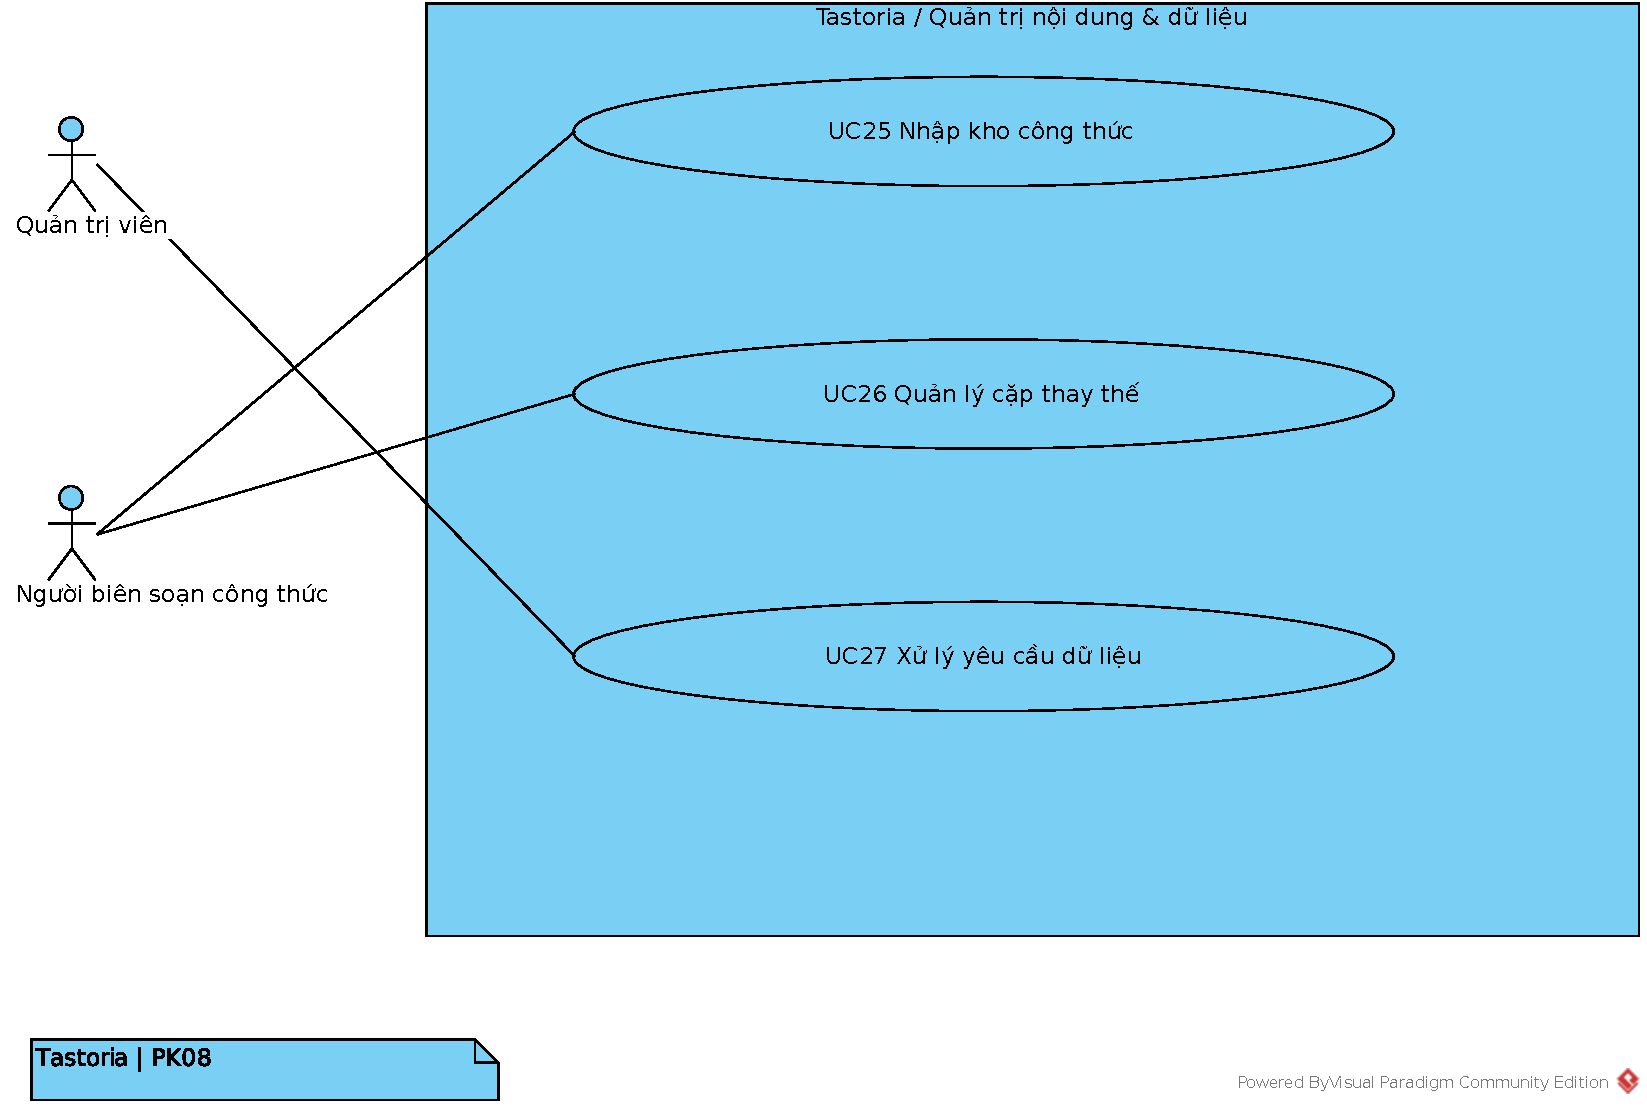
\includegraphics[width=0.96\linewidth,height=0.78\textwidth,keepaspectratio]{assets/PK08.pdf}
\caption{PK08 --- Phân rã use case}\label{fig:Phu-luc-A-Use-Cases:8}
\end{figure}
\end{landscape}\clearpage
\section{UC25 --- Nhập và kiểm tra kho công thức, nguyên liệu}
\subsection{Mục tiêu trong ngữ cảnh}
Người biên soạn công thức (A05) đưa một bộ dữ liệu (bundle YAML/\allowbreak{}CSV) gồm nguyên liệu, món, bước nấu, nguồn tham khảo vào kho món của hệ thống. Hệ thống kiểm tra toàn bộ bundle trước khi ghi, nhập trong một giao dịch, rồi tính lại dinh dưỡng món theo bảng thành phần thực phẩm. Kết quả là kho món mà UC15 (ghép mâm), UC19 (lịch nấu) và UC17 (thay thế) dùng được ngay, với mọi con số truy được về nguồn.

\subsection{Phạm vi và mức}
\begin{itemize}
\item Phạm vi: hệ thống Tastoria, module {\small\texttt{admin}} (lệnh CLI) gọi module {\small\texttt{catalog}}.
\item Mức: mục tiêu người dùng (user goal), thao tác của nhân sự qua CLI trong container {\small\texttt{api}}.
\end{itemize}
\subsection{Tác nhân và bên liên quan (quyền lợi)}
{\footnotesize\setlength{\tabcolsep}{0pt}
\begin{longtable}{@{}L{7.850cm}@{\hspace{3mm}}L{7.850cm}@{}}
\caption{Tác nhân và bên liên quan (quyền lợi)}\\
\toprule
\textbf{Bên} & \textbf{Quyền lợi} \\
\midrule\endfirsthead
\multicolumn{2}{l}{\small\itshape Bảng \thetable{} (tiếp theo)}\\
\toprule
\textbf{Bên} & \textbf{Quyền lợi} \\
\midrule\endhead
\bottomrule\endfoot
A05 Người biên soạn công thức & Nhập nhanh 150--200 món; biết chính xác dòng nào sai; không làm hỏng kho đang chạy khi bundle lỗi. \\ \addlinespace[3pt]
A02 Người dùng & Không bao giờ nhận món chứa nhóm dị ứng đã khai vì dữ liệu nguyên liệu thiếu khai báo dị ứng; calo hiển thị có nguồn. \\ \addlinespace[3pt]
A06 Người vận hành mô hình & Kho món ổn định, có phiên bản dữ liệu để tái lập thí nghiệm xếp hạng và ghép mâm. \\ \addlinespace[3pt]
Nhóm đồ án /\allowbreak{} giám khảo & Mọi món có \ensuremath{\geq} 2 nguồn, bước nấu tách chủ động/\allowbreak{}thụ động, dinh dưỡng tính theo công thức công bố (EuroFIR). \\ \addlinespace[3pt]
\end{longtable}}
\subsection{Tiền điều kiện}
\begin{enumerate}
\item A05 có quyền chạy lệnh trong container {\small\texttt{api}} trên máy chủ lab (ví dụ {\small\texttt{docker compose exec api tastoria catalog import .\allowbreak{}.\allowbreak{}.\allowbreak{}}}).
\item Dữ liệu tham chiếu đã có: {\small\texttt{nutrient\_\allowbreak{}\allowbreak{}sources}}, {\small\texttt{food\_\allowbreak{}\allowbreak{}items}}, {\small\texttt{food\_\allowbreak{}\allowbreak{}nutrients}}, {\small\texttt{nutrients}}, {\small\texttt{food\_\allowbreak{}\allowbreak{}groups}}, {\small\texttt{allergen\_\allowbreak{}\allowbreak{}groups}}, {\small\texttt{diets}}, {\small\texttt{cooking\_\allowbreak{}\allowbreak{}methods}}, {\small\texttt{tags}} (nạp ở D0 hoặc nằm trong chính bundle).
\item Thư mục bundle nằm trong container và đọc được.
\end{enumerate}
\subsection{Đảm bảo tối thiểu}
Kho món không bao giờ ở trạng thái nửa vời: hoặc toàn bộ bundle được ghi, hoặc không ghi gì. Mỗi lần chạy (thành công hay thất bại) đều có báo cáo kiểm tra in ra và một dòng {\small\texttt{audit\_\allowbreak{}\allowbreak{}log}}.

\subsection{Đảm bảo khi thành công}
\begin{enumerate}
\item Mọi nguyên liệu, món, bước, thẻ, nguồn trong bundle có mặt trong các bảng {\small\texttt{catalog}}.
\item Món {\small\texttt{published}} bị sửa được nhập thành bản mới; bản cũ chuyển {\small\texttt{retired}}, mâm và phiên nấu cũ vẫn trỏ bản cũ (BR-\allowbreak{}CATALOG-\allowbreak{}01).
\item {\small\texttt{recipe\_\allowbreak{}\allowbreak{}nutrition}} của mọi món bị ảnh hưởng được tính lại, ghi {\small\texttt{computed\_\allowbreak{}\allowbreak{}at}} và {\small\texttt{data\_\allowbreak{}\allowbreak{}version}}.
\item Kiểm tra dị ứng toàn kho (BR-\allowbreak{}ALG-\allowbreak{}01) cho kết quả 0 vi phạm.
\end{enumerate}
\subsection{Kích hoạt}
A05 chạy {\small\texttt{tastoria catalog import <bundle\_\allowbreak{}\allowbreak{}dir>}} sau khi soạn hoặc sửa bundle.

\subsection{Kịch bản chính}
\begin{enumerate}
\item A05 chạy {\small\texttt{tastoria catalog import <bundle\_\allowbreak{}\allowbreak{}dir>}}.
\item Module {\small\texttt{admin}} đọc toàn bộ tệp trong bundle, phân tích cú pháp YAML/\allowbreak{}CSV.
\item Module {\small\texttt{admin}} gọi {\small\texttt{catalog.\allowbreak{}validate\_\allowbreak{}\allowbreak{}bundle()}}; module {\small\texttt{catalog}} kiểm tra lược đồ từng bản ghi (kiểu, trường bắt buộc, giá trị enum như {\small\texttt{slot \ensuremath{\in} \{man, rau, canh\}}}, {\small\texttt{kind \ensuremath{\in} \{active, passive\}}}).
\item Module {\small\texttt{catalog}} kiểm tra tham chiếu: nhóm thực phẩm, nhóm dị ứng, cách nấu, thẻ, nguồn thành phần ({\small\texttt{comp\_\allowbreak{}\allowbreak{}source\_\allowbreak{}\allowbreak{}id}}, {\small\texttt{comp\_\allowbreak{}\allowbreak{}source\_\allowbreak{}\allowbreak{}code}} trỏ đúng {\small\texttt{food\_\allowbreak{}\allowbreak{}items}}), nguyên liệu trong món đã tồn tại hoặc có trong bundle.
\item Module {\small\texttt{catalog}} kiểm tra quy tắc nghiệp vụ: mỗi nguyên liệu khai báo tường minh danh sách nhóm dị ứng (có thể rỗng); nguyên liệu đếm được có ít nhất một dòng quy đổi đơn vị; thời hạn ngăn mát có căn cứ; món có \ensuremath{\geq} 2 nguồn, bước đánh số liên tục, phút > 0; gam > 0.
\item Module {\small\texttt{catalog}} so bundle với kho hiện có, lập danh sách thay đổi: thêm mới, cập nhật bản {\small\texttt{draft}}, tạo bản mới cho món {\small\texttt{published}} bị sửa, ngừng dùng ({\small\texttt{is\_\allowbreak{}\allowbreak{}active=false}} /\allowbreak{} {\small\texttt{retired}}).
\item Module {\small\texttt{admin}} mở một Unit of Work (module {\small\texttt{core}}) và gọi {\small\texttt{catalog.\allowbreak{}apply\_\allowbreak{}\allowbreak{}bundle()}}; module {\small\texttt{catalog}} ghi các bảng theo danh sách thay đổi.
\item Module {\small\texttt{catalog}} tính lại {\small\texttt{recipe\_\allowbreak{}\allowbreak{}nutrition}} cho mọi món mới hoặc bị ảnh hưởng theo BR-\allowbreak{}NUT-\allowbreak{}05.
\item Module {\small\texttt{catalog}} chạy kiểm tra dị ứng và chế độ ăn toàn kho trên dữ liệu vừa ghi (cùng giao dịch).
\item Module {\small\texttt{admin}} gọi {\small\texttt{privacy.\allowbreak{}record\_\allowbreak{}\allowbreak{}audit()}} ghi {\small\texttt{audit\_\allowbreak{}\allowbreak{}log}} (action {\small\texttt{catalog.\allowbreak{}import}}, actor\_\allowbreak{}role {\small\texttt{curator}}).
\item Unit of Work commit. Module {\small\texttt{admin}} in báo cáo: số bản ghi thêm/\allowbreak{}sửa/\allowbreak{}ngừng theo bảng, số món tính lại dinh dưỡng, {\small\texttt{data\_\allowbreak{}\allowbreak{}version}}, thời gian chạy; thoát mã 0.
\end{enumerate}
\subsection{Mở rộng}
\begin{itemize}
\item \textbf{2a. Bundle không đọc được} (thư mục không tồn tại, tệp không phải UTF-\allowbreak{}8, YAML sai cú pháp): {\small\texttt{admin}} in tệp và dòng lỗi, thoát mã \ensuremath{\neq} 0, không mở giao dịch, vẫn ghi {\small\texttt{audit\_\allowbreak{}\allowbreak{}log}} với kết quả thất bại.
\item \textbf{3a. Lỗi lược đồ hoặc enum} (lỗi nhập): {\small\texttt{catalog}} gom mọi lỗi (không dừng ở lỗi đầu), {\small\texttt{admin}} in danh sách {\small\texttt{tệp:dòng: mã lỗi: mô tả}}, thoát mã \ensuremath{\neq} 0, không ghi gì vào kho.
\item \textbf{4a. Tham chiếu không tồn tại} (ví dụ nhóm dị ứng hoặc mã {\small\texttt{food\_\allowbreak{}\allowbreak{}items}} không có): như 3a.
\item \textbf{5a. Nguyên liệu thiếu khai báo dị ứng}: lỗi chặn (BR-\allowbreak{}ALG-\allowbreak{}01, BR-\allowbreak{}ALG-\allowbreak{}02); như 3a.
\item \textbf{5b. Món có < 2 nguồn hoặc nguyên liệu chưa ánh xạ bảng thành phần}: món có thể nhập ở trạng thái {\small\texttt{draft}} nhưng không được chuyển {\small\texttt{published}}; báo lỗi nếu bundle khai {\small\texttt{published}}.
\item \textbf{6a. Bundle sửa nguyên liệu hoặc bước của món {\small\texttt{published}}}: {\small\texttt{catalog}} tạo bản ghi {\small\texttt{recipes}} mới (id mới, {\small\texttt{published}}) và chuyển bản cũ sang {\small\texttt{retired}} (BR-\allowbreak{}CATALOG-\allowbreak{}01); báo cáo liệt kê cặp id cũ \ensuremath{\rightarrow} mới.
\item \textbf{6b. Bundle bỏ một nguyên liệu hoặc món đang có}: không xoá cứng; nguyên liệu chuyển {\small\texttt{is\_\allowbreak{}\allowbreak{}active=false}}, món chuyển {\small\texttt{retired}} (BR-\allowbreak{}CATALOG-\allowbreak{}01).
\item \textbf{6c. Bundle giống hệt kho hiện có} (chạy lại lũy đẳng): danh sách thay đổi rỗng; không tạo bản mới, không tính lại dinh dưỡng; báo cáo "0 thay đổi"; thoát mã 0.
\item \textbf{8a. Không tính được dinh dưỡng một món} (nguyên liệu không có giá trị {\small\texttt{energy\_\allowbreak{}\allowbreak{}kcal}} trong nguồn): lỗi chặn với món {\small\texttt{published}}; giao dịch rollback; báo cáo chỉ ra nguyên liệu và chất thiếu.
\item \textbf{9a. Kiểm tra dị ứng toàn kho phát hiện vi phạm}: rollback toàn bộ; báo cáo liệt kê (món, nguyên liệu, nhóm dị ứng).
\item \textbf{7a. Lỗi hệ thống giữa chừng} (mất kết nối DB, container bị dừng): giao dịch rollback; kho giữ nguyên bản trước; A05 chạy lại cùng lệnh (an toàn vì 6c).
\item \textbf{*a. Quá thời gian}: lệnh không có giới hạn thời gian cứng; nếu A05 ngắt (Ctrl+C) trước bước 11 thì giao dịch rollback như 7a.
\item Quan hệ include/\allowbreak{}extend: model.yaml không khai báo include/\allowbreak{}extend cho UC25.
\end{itemize}
\subsection{Ghi chú đối chiếu của báo cáo}
Giữ phạm vi yêu cầu của đặc tả nguồn; cần kiểm thử theo môi trường và phiên bản thực tế trước khi ghi kết quả nghiệm thu.

\textbf{Nguồn:} {\small\texttt{Tastoria/\allowbreak{}\allowbreak{}docs/\allowbreak{}\allowbreak{}sad/\allowbreak{}\allowbreak{}use-\allowbreak{}cases/\allowbreak{}\allowbreak{}UC25.\allowbreak{}md}}. Mã nghiệp vụ: BR-\allowbreak{}NUT-\allowbreak{}05, BR-\allowbreak{}ALG-\allowbreak{}01, BR-\allowbreak{}ALG-\allowbreak{}02, BR-\allowbreak{}CATALOG-\allowbreak{}01, BR-\allowbreak{}QTY-\allowbreak{}02, BR-\allowbreak{}FRESH-\allowbreak{}01, BR-\allowbreak{}DIET-\allowbreak{}01, BR-\allowbreak{}TRAY-\allowbreak{}01, BR-\allowbreak{}COOK-\allowbreak{}01.

\textbf{Dữ liệu liên quan:} {\small\texttt{recipes}}, {\small\texttt{recipe\_\allowbreak{}\allowbreak{}ingredients}}, {\small\texttt{recipe\_\allowbreak{}\allowbreak{}steps}}, {\small\texttt{recipe\_\allowbreak{}\allowbreak{}tags}}, {\small\texttt{recipe\_\allowbreak{}\allowbreak{}sources}}, {\small\texttt{recipe\_\allowbreak{}\allowbreak{}nutrition}}, {\small\texttt{ingredients}}, {\small\texttt{ingredient\_\allowbreak{}\allowbreak{}synonyms}}, {\small\texttt{ingredient\_\allowbreak{}\allowbreak{}allergens}}, {\small\texttt{ingredient\_\allowbreak{}\allowbreak{}units}}, {\small\texttt{food\_\allowbreak{}\allowbreak{}items}}, {\small\texttt{food\_\allowbreak{}\allowbreak{}nutrients}}, {\small\texttt{nutrient\_\allowbreak{}\allowbreak{}sources}}, {\small\texttt{nutrients}}, {\small\texttt{food\_\allowbreak{}\allowbreak{}groups}}, {\small\texttt{allergen\_\allowbreak{}\allowbreak{}groups}}, {\small\texttt{diets}}, {\small\texttt{diet\_\allowbreak{}\allowbreak{}exclusions}}, {\small\texttt{qty\_\allowbreak{}\allowbreak{}levels}}, {\small\texttt{cooking\_\allowbreak{}\allowbreak{}methods}}, {\small\texttt{tags}}, {\small\texttt{audit\_\allowbreak{}\allowbreak{}log}}.

\textbf{Điểm giao tiếp:} {\small\texttt{CLI tastoria catalog import <bundle\_\allowbreak{}\allowbreak{}dir>}}.

\section{UC26 --- Quản lý cặp thay thế nguyên liệu}
\subsection{Mục tiêu trong ngữ cảnh}
Người biên soạn công thức (A05) duy trì bảng tra cặp thay thế nguyên liệu tiếng Việt có ngữ cảnh (slot, cách nấu), tỉ lệ quy đổi và nguồn. Bảng này là nguồn ứng viên (a) ở spec \S{}6.3: ghép mâm tự động chỉ dùng nguồn này, và màn "Thiếu gì?" (UC17) dùng nó trước Word2Vec. A05 soạn tệp, hệ thống kiểm tra và đồng bộ tệp vào {\small\texttt{substitution\_\allowbreak{}\allowbreak{}pairs}}.

\subsection{Phạm vi và mức}
\begin{itemize}
\item Phạm vi: hệ thống Tastoria, module {\small\texttt{admin}} (CLI) gọi module {\small\texttt{substitute}} và {\small\texttt{catalog}}.
\item Mức: mục tiêu người dùng, thao tác nhân sự qua CLI.
\end{itemize}
\subsection{Tác nhân và bên liên quan (quyền lợi)}
{\footnotesize\setlength{\tabcolsep}{0pt}
\begin{longtable}{@{}L{7.850cm}@{\hspace{3mm}}L{7.850cm}@{}}
\caption{Tác nhân và bên liên quan (quyền lợi)}\\
\toprule
\textbf{Bên} & \textbf{Quyền lợi} \\
\midrule\endfirsthead
\multicolumn{2}{l}{\small\itshape Bảng \thetable{} (tiếp theo)}\\
\toprule
\textbf{Bên} & \textbf{Quyền lợi} \\
\midrule\endhead
\bottomrule\endfoot
A05 Người biên soạn công thức & Sửa bảng tra bằng một tệp, biết ngay cặp nào sai. \\ \addlinespace[3pt]
A02 Người dùng & Gợi ý thay thế hợp ngữ cảnh món; không bao giờ nhận đồ thay thế thuộc nhóm dị ứng của mình (lọc ở UC17, UC15). \\ \addlinespace[3pt]
A06 Người vận hành mô hình & Bảng tra là baseline và nguồn chính để đánh giá thay thế (Hit@1/\allowbreak{}3, MRR); cần ổn định và có nguồn. \\ \addlinespace[3pt]
\end{longtable}}
\subsection{Tiền điều kiện}
\begin{enumerate}
\item A05 có quyền chạy lệnh trong container {\small\texttt{api}}.
\item Nguyên liệu nhắc tới trong tệp đã có trong {\small\texttt{ingredients}} (nhập bằng UC25).
\end{enumerate}
\subsection{Đảm bảo tối thiểu}
Bảng {\small\texttt{substitution\_\allowbreak{}\allowbreak{}pairs}} hoặc được cập nhật trọn tệp, hoặc giữ nguyên. Mọi lần chạy có báo cáo và một dòng {\small\texttt{audit\_\allowbreak{}\allowbreak{}log}}.

\subsection{Đảm bảo khi thành công}
\begin{enumerate}
\item Mọi cặp {\small\texttt{curated = true}} trong {\small\texttt{substitution\_\allowbreak{}\allowbreak{}pairs}} khớp đúng nội dung tệp (thêm, sửa {\small\texttt{ratio}}/\allowbreak{}{\small\texttt{score}}/\allowbreak{}{\small\texttt{source}}, xoá cặp không còn trong tệp).
\item Cặp {\small\texttt{curated = false}} (sinh từ nguồn khác) không bị đụng.
\item Không cặp nào vi phạm: tự thay chính nó, khác nhóm thực phẩm, trỏ nguyên liệu ngừng dùng.
\end{enumerate}
\subsection{Kích hoạt}
A05 chạy {\small\texttt{tastoria catalog substitutes import <file>}}.

\subsection{Kịch bản chính}
\begin{enumerate}
\item A05 chạy {\small\texttt{tastoria catalog substitutes import <file>}}.
\item Module {\small\texttt{admin}} đọc tệp (CSV/\allowbreak{}YAML), mỗi dòng gồm: nguyên liệu gốc, nguyên liệu thay, {\small\texttt{context\_\allowbreak{}\allowbreak{}slot}} (tuỳ chọn), {\small\texttt{context\_\allowbreak{}\allowbreak{}method\_\allowbreak{}\allowbreak{}code}} (tuỳ chọn), {\small\texttt{ratio}}, {\small\texttt{score}}, {\small\texttt{source}}.
\item Module {\small\texttt{admin}} gọi {\small\texttt{catalog}} để phân giải tên nguyên liệu ({\small\texttt{name\_\allowbreak{}\allowbreak{}vi}} hoặc {\small\texttt{ingredient\_\allowbreak{}\allowbreak{}synonyms}}) thành {\small\texttt{ingredients.\allowbreak{}id}}, kiểm {\small\texttt{cooking\_\allowbreak{}\allowbreak{}methods.\allowbreak{}code}}.
\item Module {\small\texttt{admin}} gọi {\small\texttt{substitute.\allowbreak{}validate\_\allowbreak{}\allowbreak{}pairs()}}; module {\small\texttt{substitute}} kiểm từng cặp: hai nguyên liệu khác nhau, cùng {\small\texttt{food\_\allowbreak{}\allowbreak{}group\_\allowbreak{}\allowbreak{}code}}, cả hai {\small\texttt{is\_\allowbreak{}\allowbreak{}active = true}}, {\small\texttt{ratio > 0}}, {\small\texttt{score}} trong [0, 1], {\small\texttt{source}} không rỗng, slot hợp lệ, không trùng khoá (gốc, thay, slot, cách nấu) trong tệp.
\item Module {\small\texttt{substitute}} so với các cặp {\small\texttt{curated = true}} hiện có, lập danh sách thêm/\allowbreak{}sửa/\allowbreak{}xoá.
\item Module {\small\texttt{admin}} mở Unit of Work (module {\small\texttt{core}}), gọi {\small\texttt{substitute.\allowbreak{}apply\_\allowbreak{}\allowbreak{}curated\_\allowbreak{}\allowbreak{}pairs()}} ghi {\small\texttt{substitution\_\allowbreak{}\allowbreak{}pairs}}.
\item Module {\small\texttt{admin}} gọi {\small\texttt{privacy.\allowbreak{}record\_\allowbreak{}\allowbreak{}audit()}} ghi {\small\texttt{audit\_\allowbreak{}\allowbreak{}log}} (action {\small\texttt{substitutes.\allowbreak{}import}}, actor\_\allowbreak{}role {\small\texttt{curator}}).
\item Unit of Work commit; {\small\texttt{admin}} in báo cáo số cặp thêm/\allowbreak{}sửa/\allowbreak{}xoá; thoát mã 0.
\end{enumerate}
\subsection{Mở rộng}
\begin{itemize}
\item \textbf{2a. Tệp không đọc được hoặc sai cú pháp}: in vị trí lỗi, thoát mã \ensuremath{\neq} 0, không ghi gì; ghi {\small\texttt{audit\_\allowbreak{}\allowbreak{}log}} thất bại.
\item \textbf{3a. Tên nguyên liệu không phân giải được hoặc phân giải ra nhiều id} (lỗi nhập): lỗi chặn cho dòng đó; gom mọi lỗi, thoát mã \ensuremath{\neq} 0, không ghi gì.
\item \textbf{4a. Cặp tự thay chính nó}: lỗi chặn (khớp ràng buộc CK {\small\texttt{ingredient\_\allowbreak{}\allowbreak{}id <> substitute\_\allowbreak{}\allowbreak{}id}}).
\item \textbf{4b. Hai nguyên liệu khác nhóm thực phẩm}: lỗi chặn (spec \S{}6.3: lọc cứng cùng nhóm).
\item \textbf{4c. Nguyên liệu {\small\texttt{is\_\allowbreak{}\allowbreak{}active = false}}}: lỗi chặn; A05 phải nhập lại nguyên liệu hoặc bỏ cặp (BR-\allowbreak{}CATALOG-\allowbreak{}01: nguyên liệu không bị xoá nên id vẫn tồn tại).
\item \textbf{4d. Trùng khoá trong tệp}: lỗi chặn, in cả hai dòng.
\item \textbf{5a. Tệp giống hệt dữ liệu hiện có} (chạy lại lũy đẳng): 0 thay đổi, thoát mã 0.
\item \textbf{6a. Lỗi hệ thống giữa chừng}: rollback; bảng giữ nguyên; chạy lại an toàn nhờ 5a.
\item \textbf{*a. Mâm hoặc thay thế đã chấp nhận trỏ tới cặp bị xoá}: không ảnh hưởng; {\small\texttt{meal\_\allowbreak{}\allowbreak{}plan\_\allowbreak{}\allowbreak{}item\_\allowbreak{}\allowbreak{}substitutions}} lưu cặp nguyên liệu, không trỏ {\small\texttt{substitution\_\allowbreak{}\allowbreak{}pairs}}.
\item Quan hệ include/\allowbreak{}extend: model.yaml không khai báo include/\allowbreak{}extend cho UC26.
\end{itemize}
\subsection{Ghi chú đối chiếu của báo cáo}
Giữ phạm vi yêu cầu của đặc tả nguồn; cần kiểm thử theo môi trường và phiên bản thực tế trước khi ghi kết quả nghiệm thu.

\textbf{Nguồn:} {\small\texttt{Tastoria/\allowbreak{}\allowbreak{}docs/\allowbreak{}\allowbreak{}sad/\allowbreak{}\allowbreak{}use-\allowbreak{}cases/\allowbreak{}\allowbreak{}UC26.\allowbreak{}md}}. Mã nghiệp vụ: BR-\allowbreak{}ALG-\allowbreak{}01, BR-\allowbreak{}CATALOG-\allowbreak{}01, BR-\allowbreak{}TRAY-\allowbreak{}01.

\textbf{Dữ liệu liên quan:} {\small\texttt{substitution\_\allowbreak{}\allowbreak{}pairs}}, {\small\texttt{ingredients}}, {\small\texttt{cooking\_\allowbreak{}\allowbreak{}methods}}, {\small\texttt{food\_\allowbreak{}\allowbreak{}groups}}, {\small\texttt{audit\_\allowbreak{}\allowbreak{}log}}.

\textbf{Điểm giao tiếp:} {\small\texttt{CLI tastoria catalog substitutes import <file>}}.

\section{UC27 --- Xử lý yêu cầu dữ liệu và xem nhật ký kiểm toán}
\subsection{Mục tiêu trong ngữ cảnh}
Quản trị viên (A04) xem hàng đợi yêu cầu của chủ thể dữ liệu ({\small\texttt{dsr\_\allowbreak{}\allowbreak{}requests}}), xử lý thủ công các yêu cầu hệ thống không tự hoàn tất (sửa, hạn chế, phản đối --- từ UC08) hoặc bị kẹt, ghi kết quả và lý do; đồng thời tra {\small\texttt{audit\_\allowbreak{}\allowbreak{}log}} để chứng minh ai đã giải mã dữ liệu sức khoẻ hay thao tác dữ liệu nào. Mục tiêu là mọi yêu cầu hoàn tất trong hạn và có bằng chứng kiểm chứng được.

\subsection{Phạm vi và mức}
\begin{itemize}
\item Phạm vi: hệ thống Tastoria, module {\small\texttt{admin}} gọi module {\small\texttt{privacy}} và {\small\texttt{identity}}.
\item Mức: mục tiêu người dùng, giao diện API nhân sự ({\small\texttt{staff:admin}}).
\end{itemize}
\subsection{Tác nhân và bên liên quan (quyền lợi)}
{\footnotesize\setlength{\tabcolsep}{0pt}
\begin{longtable}{@{}L{7.850cm}@{\hspace{3mm}}L{7.850cm}@{}}
\caption{Tác nhân và bên liên quan (quyền lợi)}\\
\toprule
\textbf{Bên} & \textbf{Quyền lợi} \\
\midrule\endfirsthead
\multicolumn{2}{l}{\small\itshape Bảng \thetable{} (tiếp theo)}\\
\toprule
\textbf{Bên} & \textbf{Quyền lợi} \\
\midrule\endhead
\bottomrule\endfoot
A04 Quản trị viên & Thấy ngay yêu cầu nào sắp/\allowbreak{}đã quá hạn; ghi kết quả một lần, không thao tác trùng. \\ \addlinespace[3pt]
A02 Người dùng (chủ thể dữ liệu) & Yêu cầu tự động hoàn tất \ensuremath{\leq} 24 giờ; yêu cầu thủ công được xác nhận \ensuremath{\leq} 24 giờ và hoàn tất trong hạn theo loại (BR-\allowbreak{}DSR-\allowbreak{}01); xem được trạng thái qua {\small\texttt{GET /\allowbreak{}\allowbreak{}me/\allowbreak{}\allowbreak{}data-\allowbreak{}requests/\allowbreak{}\allowbreak{}\{id\}}}. \\ \addlinespace[3pt]
Bên kiểm soát dữ liệu (nhóm đồ án) & Có bằng chứng xử lý và nhật ký truy cập dữ liệu nhạy cảm khi bị kiểm tra. \\ \addlinespace[3pt]
\end{longtable}}
\subsection{Tiền điều kiện}
\begin{enumerate}
\item A04 đã đăng nhập (UC02) bằng tài khoản {\small\texttt{users.\allowbreak{}role = admin}}, có access token còn hạn.
\item Có ít nhất một bản ghi {\small\texttt{dsr\_\allowbreak{}\allowbreak{}requests}} hoặc {\small\texttt{audit\_\allowbreak{}\allowbreak{}log}} (nếu không, danh sách rỗng).
\end{enumerate}
\subsection{Đảm bảo tối thiểu}
Không có thay đổi trạng thái yêu cầu nào mà không có {\small\texttt{audit\_\allowbreak{}\allowbreak{}log}} tương ứng. Người không phải {\small\texttt{admin}} không đọc được hàng đợi hay nhật ký.

\subsection{Đảm bảo khi thành công}
\begin{enumerate}
\item Yêu cầu được xử lý chuyển {\small\texttt{completed}} hoặc {\small\texttt{rejected}}, có {\small\texttt{completed\_\allowbreak{}\allowbreak{}at}} và {\small\texttt{note}}.
\item Hành động xem danh sách, xem nhật ký và xử lý đều được ghi {\small\texttt{audit\_\allowbreak{}\allowbreak{}log}} (actor\_\allowbreak{}role {\small\texttt{admin}}).
\end{enumerate}
\subsection{Kích hoạt}
A04 mở hàng đợi yêu cầu (định kỳ hằng ngày hoặc khi có yêu cầu thủ công mới từ UC08), hoặc cần tra nhật ký kiểm toán.

\subsection{Kịch bản chính}
\begin{enumerate}
\item A04 gọi {\small\texttt{GET /\allowbreak{}\allowbreak{}admin/\allowbreak{}\allowbreak{}data-\allowbreak{}requests}} (lọc theo {\small\texttt{status}}, {\small\texttt{type}}).
\item Module {\small\texttt{admin}} kiểm vai trò {\small\texttt{admin}} (module {\small\texttt{identity}}), gọi {\small\texttt{privacy.\allowbreak{}list\_\allowbreak{}\allowbreak{}dsr\_\allowbreak{}\allowbreak{}requests()}}; trả danh sách phân trang keyset (created\_\allowbreak{}at, id) gồm id, type, status, received\_\allowbreak{}at, acknowledged\_\allowbreak{}at, hạn xử lý, cờ quá hạn; không trả dữ liệu sức khoẻ.
\item Module {\small\texttt{admin}} gọi {\small\texttt{privacy.\allowbreak{}record\_\allowbreak{}\allowbreak{}audit()}} ghi lượt xem.
\item A04 chọn một yêu cầu {\small\texttt{received}} hoặc {\small\texttt{in\_\allowbreak{}\allowbreak{}progress}} loại {\small\texttt{correct}}, {\small\texttt{restrict}} hoặc {\small\texttt{object}}, đọc nội dung yêu cầu.
\item A04 thực hiện việc cần làm theo quy trình nội bộ, rồi gọi {\small\texttt{POST /\allowbreak{}\allowbreak{}admin/\allowbreak{}\allowbreak{}data-\allowbreak{}requests/\allowbreak{}\allowbreak{}\{id\}/\allowbreak{}\allowbreak{}resolve}} với kết quả ({\small\texttt{in\_\allowbreak{}\allowbreak{}progress}}, {\small\texttt{completed}} hoặc {\small\texttt{rejected}}) và ghi chú.
\item Module {\small\texttt{admin}} gọi {\small\texttt{privacy.\allowbreak{}resolve\_\allowbreak{}\allowbreak{}dsr\_\allowbreak{}\allowbreak{}request()}}; module {\small\texttt{privacy}} kiểm chuyển trạng thái hợp lệ (received \ensuremath{\rightarrow} in\_\allowbreak{}progress \ensuremath{\rightarrow} completed |\allowbreak{} rejected), đặt {\small\texttt{acknowledged\_\allowbreak{}\allowbreak{}at}} nếu chưa có, đặt {\small\texttt{completed\_\allowbreak{}\allowbreak{}at}} khi kết thúc, lưu {\small\texttt{note}}.
\item Với yêu cầu {\small\texttt{restrict}} hoặc {\small\texttt{object}} được chấp nhận đối với một mục đích đồng ý, module {\small\texttt{privacy}} ghi {\small\texttt{consent\_\allowbreak{}\allowbreak{}events}} action {\small\texttt{withdraw}} và tăng {\small\texttt{users.\allowbreak{}token\_\allowbreak{}\allowbreak{}version}} qua module {\small\texttt{identity}} (BR-\allowbreak{}CONSENT-\allowbreak{}04).
\item Module {\small\texttt{privacy}} ghi {\small\texttt{audit\_\allowbreak{}\allowbreak{}log}} (action {\small\texttt{dsr.\allowbreak{}resolve}}, entity {\small\texttt{dsr\_\allowbreak{}\allowbreak{}requests}}, entity\_\allowbreak{}id).
\item Hệ thống trả trạng thái mới; A02 thấy kết quả qua {\small\texttt{GET /\allowbreak{}\allowbreak{}me/\allowbreak{}\allowbreak{}data-\allowbreak{}requests/\allowbreak{}\allowbreak{}\{id\}}}.
\item A04 gọi {\small\texttt{GET /\allowbreak{}\allowbreak{}admin/\allowbreak{}\allowbreak{}audit-\allowbreak{}log}} với bộ lọc (khoảng thời gian, actor, entity, action); module {\small\texttt{admin}} gọi {\small\texttt{privacy.\allowbreak{}list\_\allowbreak{}\allowbreak{}audit\_\allowbreak{}\allowbreak{}log()}} trả trang keyset; ghi {\small\texttt{audit\_\allowbreak{}\allowbreak{}log}} lượt tra.
\end{enumerate}
\subsection{Mở rộng}
\begin{itemize}
\item \textbf{1a. Token không hợp lệ hoặc hết hạn}: 401 {\small\texttt{application/\allowbreak{}\allowbreak{}problem+json}}; app làm mới phiên (UC02).
\item \textbf{1b. Người gọi không có vai trò {\small\texttt{admin}}} (ví dụ {\small\texttt{curator}}): 403, không trả dữ liệu, ghi {\small\texttt{audit\_\allowbreak{}\allowbreak{}log}} lượt bị từ chối.
\item \textbf{2a. Có yêu cầu quá hạn} (BR-\allowbreak{}DSR-\allowbreak{}01; hạn 24 giờ với loại tự động, hạn theo loại với loại thủ công --- FR-\allowbreak{}27-\allowbreak{}03): danh sách đánh dấu quá hạn và xếp lên đầu.
\item \textbf{5a. Từ chối không có ghi chú} (lỗi nhập): 422, trạng thái không đổi.
\item \textbf{5b. Chuyển trạng thái không hợp lệ} (ví dụ yêu cầu đã {\small\texttt{completed}}): 409, trạng thái không đổi.
\item \textbf{5c. Mất mạng sau khi gửi, A04 gửi lại cùng nội dung} (lũy đẳng): yêu cầu đã ở đúng trạng thái đích với cùng kết quả \ensuremath{\rightarrow} 200 trả trạng thái hiện tại, không ghi thêm {\small\texttt{audit\_\allowbreak{}\allowbreak{}log}} thay đổi trạng thái.
\item \textbf{5d. Yêu cầu không tồn tại}: 404.
\item \textbf{5e. Yêu cầu loại {\small\texttt{correct}} cần sửa dữ liệu hồ sơ}: module {\small\texttt{admin}} không được gọi {\small\texttt{profile}} (model.yaml); A04 hướng dẫn A02 tự sửa qua UC10 rồi đóng yêu cầu {\small\texttt{completed}} với ghi chú (xem mục 16).
\item \textbf{6a. Chủ thể đã xoá tài khoản} ({\small\texttt{user\_\allowbreak{}\allowbreak{}id}} NULL): vẫn đóng được yêu cầu; nhận diện qua {\small\texttt{subject\_\allowbreak{}\allowbreak{}ref}}.
\item \textbf{7a. Lỗi hệ thống khi ghi}: giao dịch rollback (Unit of Work), trả 500 problem+json; A04 gửi lại (5c).
\item \textbf{10a. Bộ lọc thời gian sai định dạng}: 422.
\item \textbf{*a. Quá thời gian xử lý}: yêu cầu chưa đóng sau hạn của loại hiện quá hạn (2a); hạn pháp lý theo NĐ 356/\allowbreak{}2025 Điều 5 vẫn là giới hạn ngoài cùng.
\item Quan hệ include/\allowbreak{}extend: model.yaml không khai báo include/\allowbreak{}extend cho UC27; UC08 tạo các yêu cầu thủ công mà UC27 xử lý (cùng endpoint {\small\texttt{POST /\allowbreak{}\allowbreak{}admin/\allowbreak{}\allowbreak{}data-\allowbreak{}requests/\allowbreak{}\allowbreak{}\{id\}/\allowbreak{}\allowbreak{}resolve}}).
\end{itemize}
\subsection{Ghi chú đối chiếu của báo cáo}
Giữ phạm vi yêu cầu của đặc tả nguồn; cần kiểm thử theo môi trường và phiên bản thực tế trước khi ghi kết quả nghiệm thu.

\textbf{Nguồn:} {\small\texttt{Tastoria/\allowbreak{}\allowbreak{}docs/\allowbreak{}\allowbreak{}sad/\allowbreak{}\allowbreak{}use-\allowbreak{}cases/\allowbreak{}\allowbreak{}UC27.\allowbreak{}md}}. Mã nghiệp vụ: BR-\allowbreak{}DSR-\allowbreak{}01, BR-\allowbreak{}CONSENT-\allowbreak{}04.

\textbf{Dữ liệu liên quan:} {\small\texttt{dsr\_\allowbreak{}\allowbreak{}requests}}, {\small\texttt{audit\_\allowbreak{}\allowbreak{}log}}, {\small\texttt{users}}, {\small\texttt{consent\_\allowbreak{}\allowbreak{}events}}, {\small\texttt{v\_\allowbreak{}\allowbreak{}current\_\allowbreak{}\allowbreak{}consents}}.

\textbf{Điểm giao tiếp:} {\small\texttt{GET /\allowbreak{}\allowbreak{}admin/\allowbreak{}\allowbreak{}data-\allowbreak{}requests}}; {\small\texttt{POST /\allowbreak{}\allowbreak{}admin/\allowbreak{}\allowbreak{}data-\allowbreak{}requests/\allowbreak{}\allowbreak{}\{id\}/\allowbreak{}\allowbreak{}resolve}}; {\small\texttt{GET /\allowbreak{}\allowbreak{}admin/\allowbreak{}\allowbreak{}audit-\allowbreak{}log}}.
